\label{chapter:conceitos}
Este capítulo tem como objetivo apresentar os principais conceitos e definições abordados neste trabalho, tais como: Verificação e Validação de \textit{Software}, Propriedades de Segurança, Bounded Model Checking, Execução Simbólica e Técnicas de Compiladores.

% ----------------------------------------------------------
% Verificação e Teste de Software
% ----------------------------------------------------------

\section{Verificação e Teste de \textit{Software}}
\label{sec:vv}
Os computadores modernos consistem de componentes complexos de \textit{hardware} e \textit{software}, garantir a corretude do \textit{software} geralmente é muito mais complexo do que o \textit{hardware} \cite{dsilva:2008}, principalmente que controla nosso transporte ou infraestrutura (\citeonline{Neumann:2015} documenta centenas de casos onde falhas de \textit{software} causou problemas). Verificação e Validação de Software (V\&V) é uma área da Engenharia de \textit{Software} que auxilia no desenvolvimento de \textit{software} de qualidade. V\&V analisa (verifica) e testa \textit{software} para determinar se ele funciona adequadamente, de acordo com os seus respectivos requisitos \cite{wallace:1989}. A principal diferença entre teste e verificação é o fato de teste apenas garantir a corretude para o conjunto de casos testados enquanto a verificação utiliza modelagem matemática para garantir a corretude do \textit{software}.
 
\subsection{Verificação formal}

Métodos formais podem ser considerados como: Matemática aplicada para modelagem e análise de sistemas de informação \cite{Baier:2008}. Segundo \citeonline{Clarke:2009}, verificação formal busca validar a corretude de um programa utilizando lógica matemática. Neste contexto, um programa é um objeto matemático (usualmente composto por uma série de conjuntos) com um comportamento definido, assim a lógica matemática pode ser utilizada para descrever precisamente o que é um comportamento correto do programa. Isso torna possível utilizar modelos matemáticos de um programa e assim provar a corretude de seu comportamento. 
\par
%Logo, a 
A criação de métodos automatizados para validar a corretude de programas tem um impacto significante, visto que construção manual de uma prova de corretude pode ser complexa e essa prova manual pode não funcionar corretamente para programas grandes, devido enumeração exaustiva de estados em sistemas complexos. 


\subsection{Testes de \textit{Software}}
Testar \textit{software} é um método de checar a corretude da implementação de um sistema o experimentando, basicamente é o processo de executar um \textit{software} procurando  comportamentos incorretos. Testes não são garantidos de observar todos os comportamentos de um programa, porém, se o programa contiver apenas um caminho, obviamente é possível \cite{ding:2008}.
\par
Segundo \citeonline{ding:2008} métodos formais podem ser utilizados em teste de \textit{software}, os casos de teste podem ser gerados com eficiência e eficácia quando derivados de especificações formais. Na prática, qualidade nem sempre se refere a um \textit{software} totalmente correto em projeto, pois isso aumenta o custo de produção consideravelmente. Porém, garantir que falhas específicas estarão ausentes é uma tarefa realística e é considerada uma boa métrica para garantir qualidade \cite{dsilva:2008}.

% ----------------------------------------------------------
% Execução Simbólica
% ----------------------------------------------------------
\section{Execução Simbólica}
\label{sec:exec_simb}
A ideia da execução simbólica é a utilização de valores simbólicos, ao invés de valores reais, para representação das variáveis dos programa. Como resultado, os valores de saída de um programa podem ser representado como uma função cujo domínio são os valores simbólicos de entrada \cite{Khurshid:2003}.
\par
A execução simbólica é uma técnica para gerar dados de entrada de programas utilizando valores simbólicos ao invés de valores concretos e assim representar os valores das variáveis com expressões simbólicas. Em teste de \textit{software}, a execução simbólica é utilizada para gerar entradas para cada caminho de de execução viável de um programa. Um caminho de execução viável é uma sequência de valores booleanos, todos esses caminhos podem ser representados usando utilizando uma árvore de execução \cite{Cadar:2013}.
\par
O estado de um programa executado de forma simbólica inclui: (a) Os valores simbólicos das variáveis; (b) Uma condição de caminho (CC) e um \textit{program counter} (PC). A CC é uma fórmula booleana sem quantificadores que utiliza as entradas simbólicas, a fórmula aglomera todas as restrições que as entradas devem satisfazer para que a execução siga o caminho associado. O PC define o próximo \textit{statement} a ser executado. Uma árvore de execução simbólica exibe todos os caminhos seguidos durante a execução simbólica de um programa. Segundo \citeonline{Cadar:2013} o objetivo da execução simbólica pode ser descrito como \textit{obter um conjunto de entradas tais que todos os caminhos de execução viáveis possam ser explorados uma única vez ao executar o programa com essas entradas}. 

\subsection{Árvore de execução simbólica}
\label{sub:exec_simb_tree}
A árvore é um grafo onde seus nós representam os estados do programa e as arestas representam as transições entre os estados \cite{Khurshid:2003}, a árvore é uma forma de demonstrar os caminhos possíveis dentro de um programa, a \autoref{fig:executionTree} mostra um exemplo de uma árvore para o programa da \autoref{fig:prog_arv}.  No exemplo podemos analisar os caminhos possíveis e verificamos como certos caminhos são impossíveis de ocorrer, na linha 7 temos a codição $y > x$ porém através da árvore de execução simbólica podemos perceber que a seguinte condição:  $x:Y$, $y:X$, e a CC $X>Y$ . Para a linha 7 dar falso a condição de caminho será $(X>Y) \land (Y>X)$, o que é uma contradição.

\begin{figure}[thp]
	\caption{\label{fig:prog_arv} Exemplo de programa para execução simbólica}
	\begin{center}
    \begin{minipage}{0.6\textwidth}
    \begin{lstlisting}[language=C]       
int x,y;
  
if(x > y){
    x = x + y;
    y = x - y;
    x = y - x;
    if(y > x) {
  	  error();
    }
}
	\end{lstlisting}
    \end{minipage}
	\end{center}
    \legend{Fonte: Adaptado de \cite{Khurshid:2003}}
\end{figure}

\begin{figure}[htb]
	\caption{\label{fig:executionTree} Exemplo de árvore de execução simbólica}
	\begin{center}
	    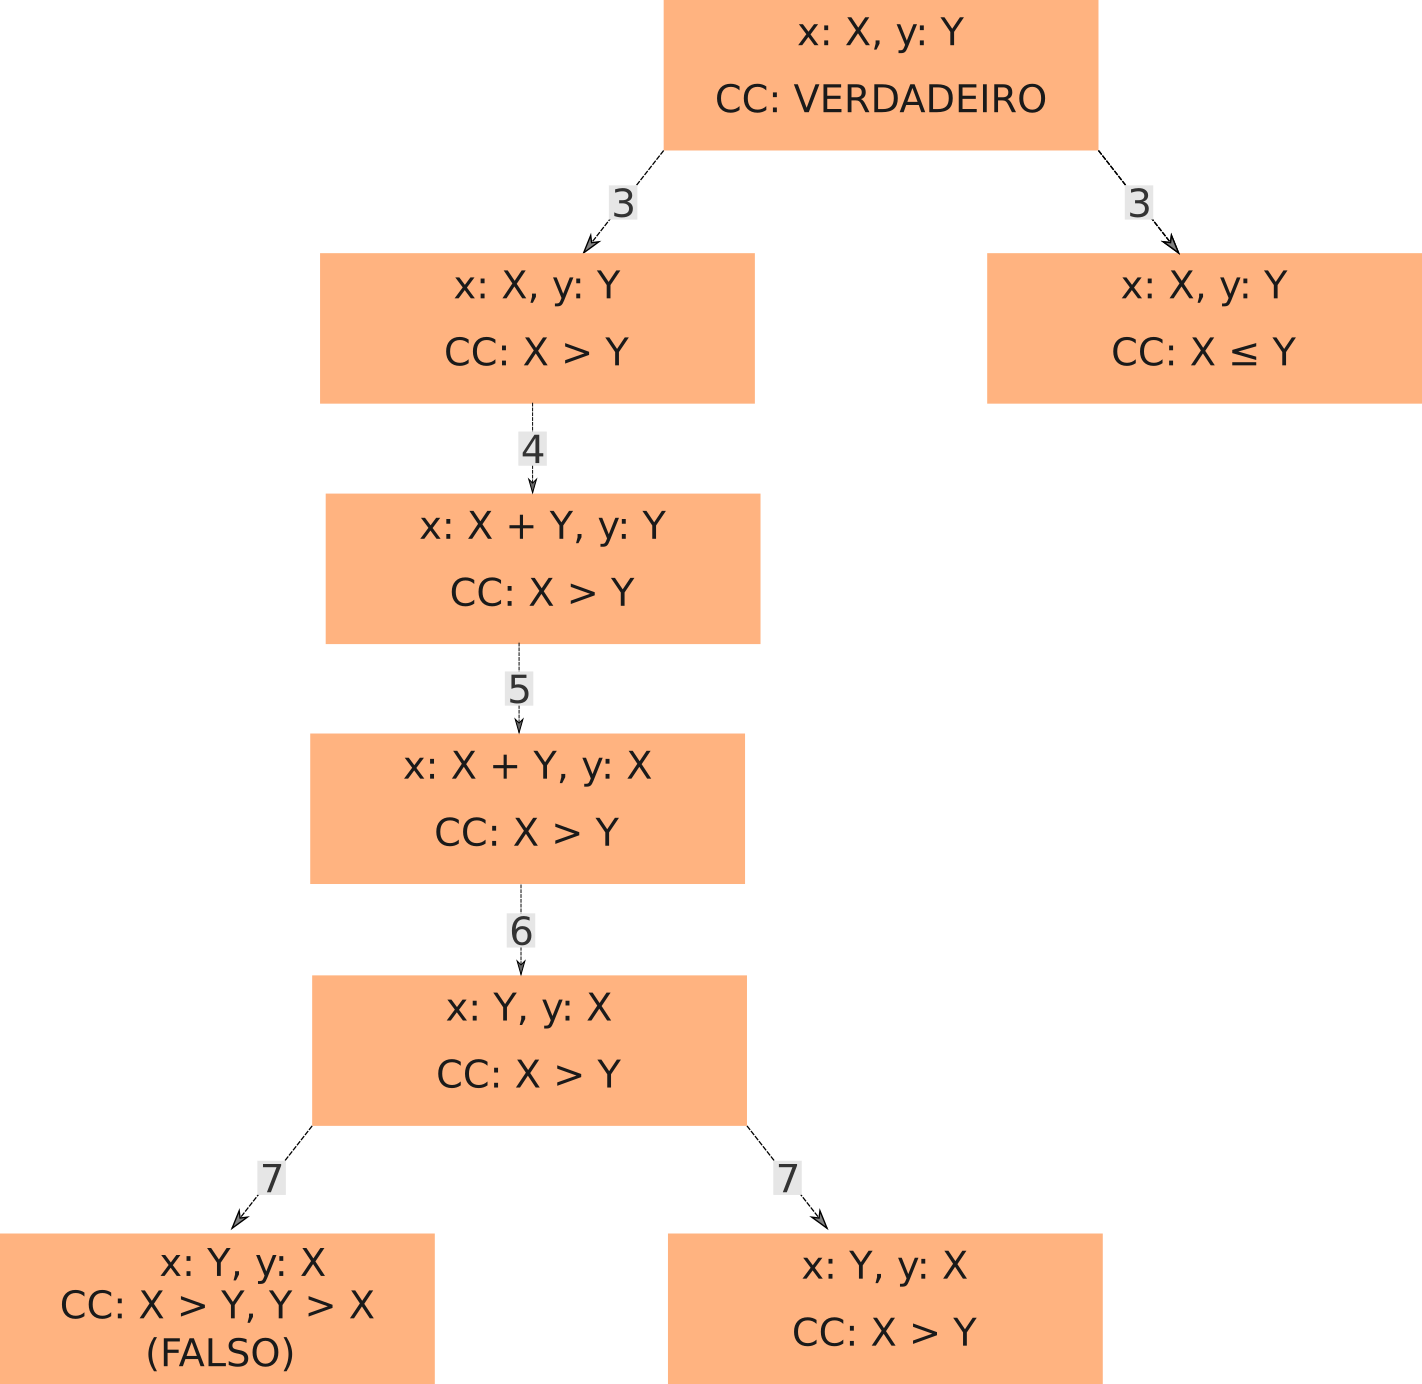
\includegraphics[scale=0.25]{resources/executionTree.png}
	\end{center}
	\legend{Fonte: Adaptado de \cite{Khurshid:2003}}
\end{figure}

% ----------------------------------------------------------
% Propriedades de Segurança
% ----------------------------------------------------------
\section{Propriedades de Segurança}
\label{sec:prop_seg}
Propriedades de segurança são imposições sobre os requerimentos de um conjunto finito de caminhos, e que, não podem ser verificados considerando apenas o estado. Um exemplo disso, seria um caixa eletrônico, um requerimento seria de que o dinheiro só pode ser retirado somente se a pessoa forneceu uma identificação válida\cite{Baier:2008}. Segundo \cite{Rocha:2015tese} podemos, informalmente, dizer que uma propriedade em tempo linear especifica um comportamento admissível de um sistema. Caso o sistema falhe ao satisfazer alguma propriedade de segurança (o usuário possa retirar dinheiro sem se identificar), então existe uma execução finita que revele isso.
\par
Formalmente podemos definir uma propriedade de segurança como: \textit{dado um sistema de transições $ST = (S, S_0, E)$, seja um conjunto $B \subset S$ que especifica um conjunto de maus estados tais que $S_0 \cap B = \emptyset$, pode-se dizer que $ST$ é seguro com relação a $B$, denotado por $ST \models AG\neg B$ se não existe um caminho no sistema de transição do estado inicial $S_0$ até o estado $B$, de outro modo é dito que $ST$ não é seguro} \cite{Rocha:2015tese}.

\subsection{Propriedades de segurança de memória}
\subsubsection{Desalocação inválida}
\subsubsection{Vazamentos de memória}
\subsubsection{Desreferência de ponteiros}

% ----------------------------------------------------------
% Bounded model checking
% ----------------------------------------------------------
\section{\textit{Bounded model checking}}
\label{sec:bmc}
Técnicas de verificação baseadas em modelo são baseadas em descrever o possível comportamento de um sistema de uma forma matemática, precisa e não ambígua. Verificou-se que uma modelagem precisa de um sistema muitas vezes leva a descoberta de incompletudes, ambiguidades e inconsistências em especificações informais. Esse problemas geralmente só são descobertos muito depois durante o processo de desenvolvimento. Os modelos de sistemas são acompanhados por algoritmos que sistematicamente exploram todos os estados de um modelo de sistema. Isso provêm a base para uma gama de técnicas de verificação indo desde exploração exaustiva (\textit{model checking}) até experimentos com um conjunto restrito de cenários no modelo (simulação), ou na realidade (testes) \cite{Baier:2008}.
\par
\textit{Model checking} é uma técnica de verificação que explora todos os estados possíveis do sistema utilizando força-bruta. Dessa maneira, o \textit{model checking} pode demonstrar que um dado modelos de sistema realmente satisfaz uma determinada propriedade. A dificuldade do \textit{model checking} é lidar com espaços de estados muito grandes, pois dependendo do sistema eles podem crescer demais  \cite{Baier:2008}. 
\par
O modelo sistema é geralmente gerado de forma automática a partir de uma descrição do modelo que é especificado em algum dialeto de linguagens de programação como C ou Java. A especificação de uma propriedade descreve o que sistema deve fazer, e o que não deve fazer, enquanto a descrição do modelo descreve como o sistema se comporta. O \textit{model checker} examina todos os estados relevantes e checa se eles satisfazem a propriedade desejada. Se um estado viola essa propriedade, o \textit{model checker} gera um contra-exemplo que indica como o modelo pode chegar em um estado indesejado \cite{Baier:2008}.
\par
Segundo \citeonline{Rocha:2015tese} o \textit{Bounded Model Checking} (BMC) é a verificação de uma dada propriedade em uma determinada profundidade: dado um sistema de transições M, uma propriedade $\phi$, e um limite (\textit{bound}) $k$, o BMC desenrola o sistema $k$ vezes e traduz o sistema em uma condição de verificação(CV) $\psi$ tal que $\psi$ é satisfeito se e somente se $\phi$ tem um contra-exemplo de profundidade menor ou igual a $k$.

% ----------------------------------------------------------
% Compilação e análise de Programas
% ----------------------------------------------------------
\section{Técnicas de Compiladores}
\label{sec:compiladores}
Esta seção irá descrever os seguintes tópicos: Análise Estática, Análise Dinâmica, Otimizações de Código e LLVM.

\subsection{Análise Estática}
A análise estática é a análise de um programa sem a execução. Compiladores utilizam esse tipo de análise durante o processo de compilação para verificar erros (como de tipagem) e otimização de código. As ferramentas que fazem essa análise só precisam ler o código para efetuar a análise \cite{Rocha:2015tese}.

\par
Um exemplo de aplicação que utiliza esse tipo de análise seria o ASTRÉE \cite{Cousot:2005} que é um analisador estático que prova automaticamente a falha de erros em tempo de execução para programas escritos em C, e foi aplicado com sucesso em vários sistemas embarcados críticos. 
%
Astrée baseia-se na teoria da interpretação abstrata \cite{Cousot:1977} e prossegue calculando uma aproximação das propriedades semânticas de traços de execução do programa analisado e provando que essas propriedades abstratas implicam na ausência de erros em tempo de execução. 
%\textcolor{red}{sua análise funciona ao aproximar rastros de propriedades semânticas de programas e provando que elas são livre de erros de execução}.

\subsection{Análise Dinâmica}
\label{sub:dinamica}
A análise dinâmica analisa a execução do programa e assim deriva propriedades de segurança para uma ou mais execuções, podendo detectar a violação das mesmas. Para a análise dinâmica, as ferramentas devem instrumentar o programa com análises \cite{Rocha:2015tese}. 

\par
O VALGRIND \cite{Nethercote:2007} é um \textit{framework} que faz uso de instrumentação binária para análise dinâmica. O módulo \textit{memcheck} VALGRIND verificar por erros de memória em tempo de execução, por exemplo, vazamentos de memória \cite{CHENG:2006}. 
%
A verificação efetuada pelo VALGRIND envolve sombrear/marcar cada bit de dados em registos e memória com um segundo \textit{bit} que indica se o bit tem um valor definido. Cada operação de determinação de valor é instrumentada com uma operação de marcação que propaga os \textit{bits} adequadamente. O Memcheck usa esses \textit{bits} de marcação para detectar usos de valores indefinidos que poderiam afetar adversamente o comportamento de um programa.


\subsection{Otimizações de Código}
\label{sub:otimization}
Podemos obter uma melhora significante no tempo de execução de um código executando otimizações locais (dentro de um bloco básico) ou através de uma otimização global (através do fluxo entre os blocos básicos) \cite{Aho:1986}. Por ser um assunto complexo e com muitas técnicas a serem consideradas, abordaremos apenas as seguintes técnicas: Representação com Grafo Acíclico Direcionado (GAD), Remoção de código morto, sub-expressões comuns, propagação de constantes.

\subsubsection{Representação com GAD}
Diversas técnicas de otimização local começam por transformar um bloco básico de código em um GAD. A \autoref{fig:gad_prog} exibe um exemplo de GAD utilizando o programa da \autoref{fig:prog_dag}. Podemos observar que os nós contém os operandos utilizados e quais variáveis se refere e já podemos vislumbrar algumas otimizações possíveis (como sub-expressões comuns), visto que $b$ e $d$ recebem os mesmos valores. 

\begin{figure}[thp]
	\caption{\label{fig:prog_dag} Exemplo de programa para geração do GAD}
	\begin{center}
    \begin{minipage}{0.5\textwidth}
    \begin{lstlisting}[language=C]       
a = b + c;
b = a - d;
c = b + c;
d = a - d;
	\end{lstlisting}
    \end{minipage}
	\end{center}
    \legend{Fonte: \cite{Aho:1986}}
\end{figure}

\begin{figure}[htb]
	\caption{\label{fig:gad_prog} Exemplo de GAD do programa da \autoref{fig:prog_dag}}
	\begin{center}
	    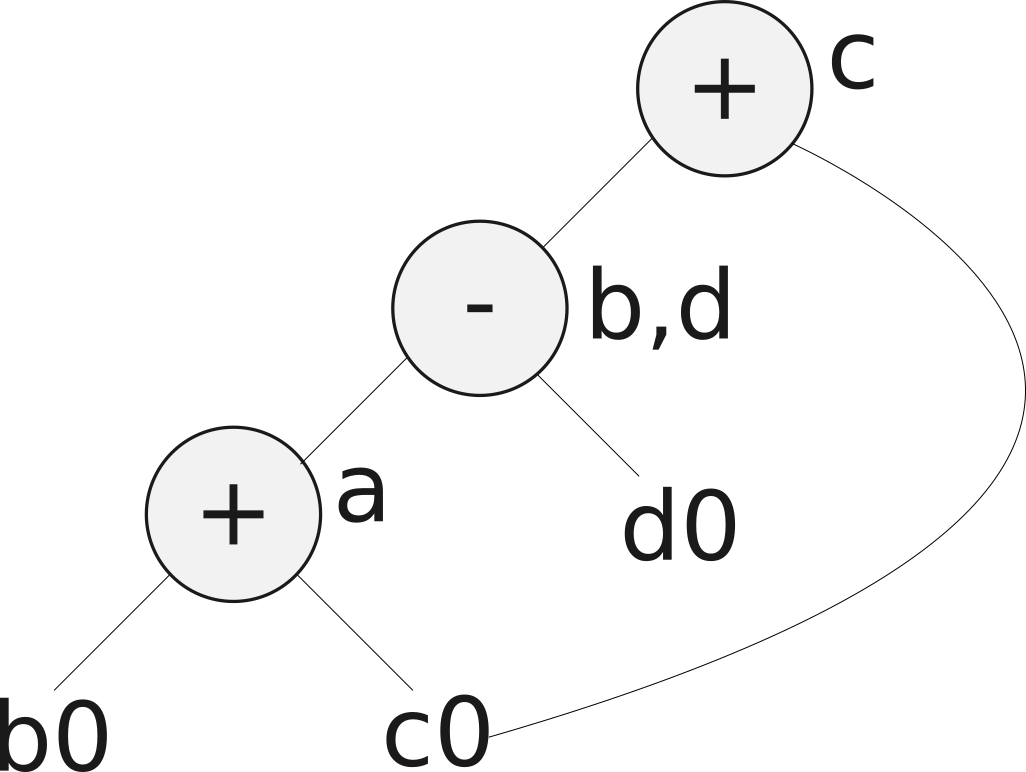
\includegraphics[scale=0.25]{resources/prog_gad.png}
	\end{center}
	\legend{Fonte: \cite{Aho:1986}}
\end{figure}

\subsubsection{Sub-expressões comuns}
Sub-expressões comuns de um programa são detectadas ao perceber que um novo nó $M$, de um GAD,  esta para ser adicionado mesmo já existindo um nó $N$ com os mesmos filhos, na mesma ordem e com os mesmos operadores. Logo, se isso ocorre, $N$ computa o mesmo valor de $M$ e pode ser usado no seu lugar \cite{Aho:1986}. No exemplo da \autoref{fig:gad_prog} podemos perceber uma otimização de sub-expressões comuns no nó atrelado a $b$ e $d$, sendo uma operação que só precisa ser realizada uma vez. A \autoref{fig:progOptimizedCommon} exibe um exemplo dessa otimização.
\begin{figure}[H]
	\caption{\label{fig:progOptimizedCommon} Programa da \autoref{fig:prog_dag} após a aplicação da técnica de sub-expressões comuns }
	\begin{center}
    \begin{minipage}{0.5\textwidth}
    \begin{lstlisting}[language=C]       
a = b + c; 
b = a - d;
c = b + c;
d = b;
	\end{lstlisting}
    \end{minipage}
	\end{center}
    \legend{Fonte: Própria}
\end{figure}

\subsubsection{Remoção de código morto}
Código morto são instruções que computam um valor que nunca será utilizado, essa técnica basicamente remove do GAD qualquer raiz que não contenha variáveis que são utilizadas em outros nós. A reaplicação dessa transformação irá remover todos os nódulos do GAD que correspondem a um código morto \cite{Aho:1986}. A \autoref{fig:progNonOptimizedDead} mostra um programa contendo algumas computações desnecessárias, como atribuições seguidas em uma variável, código inacessível, e computações cujos resultados não são utilizados.

\begin{figure}[H]
	\caption{\label{fig:progNonOptimizedDead} Programa antes da aplicação da técnica de remoção de código morto }
	\begin{center}
    \begin{minipage}{0.6\textwidth}
          \begin{lstlisting}[language=C]
int global;  

int foo() {
    int a = 3 * 7;
    int b = a / 9;
    global = 1;
    global = 10;
    return 2;
    global = 5;
}
	\end{lstlisting}
    \end{minipage}
	\end{center}
    \legend{Fonte: Própria}
  \end{figure}

  \begin{figure}[H]
	\caption{\label{fig:progOptimizedDead} Programa da \autoref{fig:progNonOptimizedDead} após a aplicação da técnica de remoção de código morto }
	\begin{center}
    \begin{minipage}{0.6\textwidth}
    \begin{lstlisting}[language=C]       
int global;  

int foo() {       
    global = 10;
    return 2;
}
	\end{lstlisting}
    \end{minipage}
	\end{center}
    \legend{Fonte: Própria}
\end{figure}

\subsubsection{Propagação de constantes}
A propagação de constantes consiste em realizar operações matemáticas ou lógicas, durante o processo de compilação ao invés de durante a execução. A técnica consiste em buscar variáveis ou funções cujo valor seja constante, ou seja, se todos os valores que sejam necessários para calcular seus valores são conhecidos durante o tempo de compilação, a computação já é executada durante a compilação \cite{Aho:1986}. A \autoref{fig:progNonOptimizedConstant} e a \autoref {fig:progOptimizedConstant} mostram como seria um programa antes e depois da aplicação dessa técnica.


\begin{figure}[H]
	\caption{\label{fig:progNonOptimizedConstant} Programa antes da aplicação da técnica de propagação de constantes }
	\begin{center}
    \begin{minipage}{0.5\textwidth}
    \begin{lstlisting}[language=C]       
int a = 2;
int b = a + 3;
	\end{lstlisting}
    \end{minipage}
	\end{center}
    \legend{Fonte: Própria}
  \end{figure}

  \begin{figure}[H]
	\caption{\label{fig:progOptimizedConstant} Programa da \autoref{fig:progNonOptimizedConstant} após a aplicação da técnica de propagação de constantes }
	\begin{center}
    \begin{minipage}{0.5\textwidth}
    \begin{lstlisting}[language=C]       
int a = 2;
int b = 5;
	\end{lstlisting}
    \end{minipage}
	\end{center}
    \legend{Fonte: Própria}
\end{figure}


\subsection{LLVM}

O LLVM é um \textit{framework} de compilação desenvolvido pra suportar de forma transparente 
e duradoura, análises e transformações de programas. Para isso, o LLVM utiliza uma linguagem intermediária, o LLVM IR e uma API em alto-nível para construção de \textit{passes} capazes de analisar ou transformar um programa em LLVM IR \cite{Lattner:2004}. 
\par
O LLVM IR consiste em um conjunto infinto de registradores virtuais que podem guardar valores de tipos primitivos (inteiro, ponto flutuante, ponteiro e booleano). 
A arquitetura do LLVM é baseada em \textit{load e store}, os programas transferem valores entre registradores e memória somente através de operações \textit{loads} e \textit{stores} usando ponteiros tipados \cite{Lattner:2004}. 
O LLVM IR utiliza instruções em um formato de \textit{Static Single Assignment} que e um formato para instruções onde para as atribuições de variáveis sempre é gerado uma nova variável para armazenar seus resultados, o que facilita otimizações e análises sobre o código \cite{Cytron:1991}, a \autoref{fig:proNonSSA} mostra um exemplo de código em C e a \autoref{fig:progSSA} mostra como ele seria no formato SSA. 
\par
O formato SSA está no paradigma funcional \cite{Appel:1998}, ou seja, um código que originalmente poderia estar em um paradigma imperativo é convertido para um paradigma funcional. A vantagem do paradigma funcional é a facilidade de realizar otimizações e análises como as descritas na \autoref{sub:otimization} \textbf{Otimizações de Código} pois: variáveis não mudam de valor, entre outras vantagens \cite{Appel:1998}. 
\par
As análise e transformações que o LLVM proporciona podem ser usadas antes ou depois do processo de linkedição, ou durante o processo de montagem (podendo gerar otimizações específicas de uma arquitetura.

\begin{figure}[H]
	\caption{\label{fig:proNonSSA} Exemplo de código C sem estar no formato SSA }
	\begin{center}
    \begin{minipage}{0.5\textwidth}
    \begin{lstlisting}[language=C]       
int a = foo();
a = a + 5;
int b = a + 3;
	\end{lstlisting}
    \end{minipage}
	\end{center}
    \legend{Fonte: Própria}
  \end{figure}

  \begin{figure}[H]
	\caption{\label{fig:progSSA}  Exemplo de código C no formato SSA }
	\begin{center}
    \begin{minipage}{0.5\textwidth}
    \begin{lstlisting}[language=C]       
int a = foo();
int a1 = a + 5; 
int b = a1 + 3;
	\end{lstlisting}
    \end{minipage}
	\end{center}
      \legend{Fonte: Própria}
  \end{figure}


% ----------------------------------------------------------
% Modelos de Memória
% ----------------------------------------------------------
\section{Modelos de Memória}

% ----------------------------------------------------------
% Invariantes de programa
% ----------------------------------------------------------
\section{Invariantes de programas}

% ----------------------------------------------------------
% Witness
% ----------------------------------------------------------
\section{\textit{Witness}}
\subsection{\textit{Witness} de violação}
\subsection{\textit{Witness} de corretude}

% ----------------------------------------------------------
% Resumo
% ----------------------------------------------------------

% \section{Resumo}
% Neste capítulo foi descrito os principais conceitos necessários para o entendimento deste trabalho. Na \autoref{sec:vv} foi definido Verificação e Teste de \textit{software} que são atividades para verificar e validar, para garantir a qualidade de um sistema. Na \autoref{sec:exec_simb} foi definido o que é execução simbólica e como ela é capaz de gerar caminhos para programas utilizando funções baseadas nos valores de entrada. Na \autoref{sec:prop_seg} foi explicado o que são propriedades de segurança e qual a importância delas para garantir que um \textit{software} esteja correto. Na \autoref{sec:bmc} foram definidos \textit{model checking} e \textit{bounded model checking} e sobre como utilizando eles é possível gerar propriedades de segurança em um programa. E finalmente, na \autoref{sec:compiladores} é comentado sobre as diversas técnicas de compiladores que são utilizadas neste trabalho.
 
